\subsection{Itération n°2}

\subsubsection{Configuration et modifications}
 
 Nous décidons de redimensionner la récompense obtenue à chaque pas de temps de sorte à ce quelle soit bornée entre $0$ et $100$. À partir de l'équation~\eqref{eq:reward}, nous déterminons que $r_{min} = r(\pi, 8, 2) \simeq -45,88$ et $r_{max} = r(0, 0, 0) = 0$. Avec ces bornes nous écrivons l'inégalité~\eqref{eq:itr2_inegalite}.
 
\begin{align}
    r_{min} &< r < 0 \label{eq:itr2_inegalite} \\
    1 &> \frac{r}{r_{min}} > 0 &&\text{car $r_{min}<0$}\\
    0 &< 1 - \frac{r}{r_{min}} < 1 &&\text{par multiplication par $-1$ puis addition de $1$}\\
    0 &< 100 \times \left( 1 - \frac{r}{r_{min}} \right) < 100 \label{eq:itr2_rescale}
\end{align}
 
Nous modifions le \emph{pendulum wrapper} pour qu'il intègre le redimensionnement de l'équation~\eqref{eq:itr2_rescale}.

\subsubsection{Analyse}

\begin{figure}[H]
    \centering
    \begin{subfigure}{0.3\textwidth}
        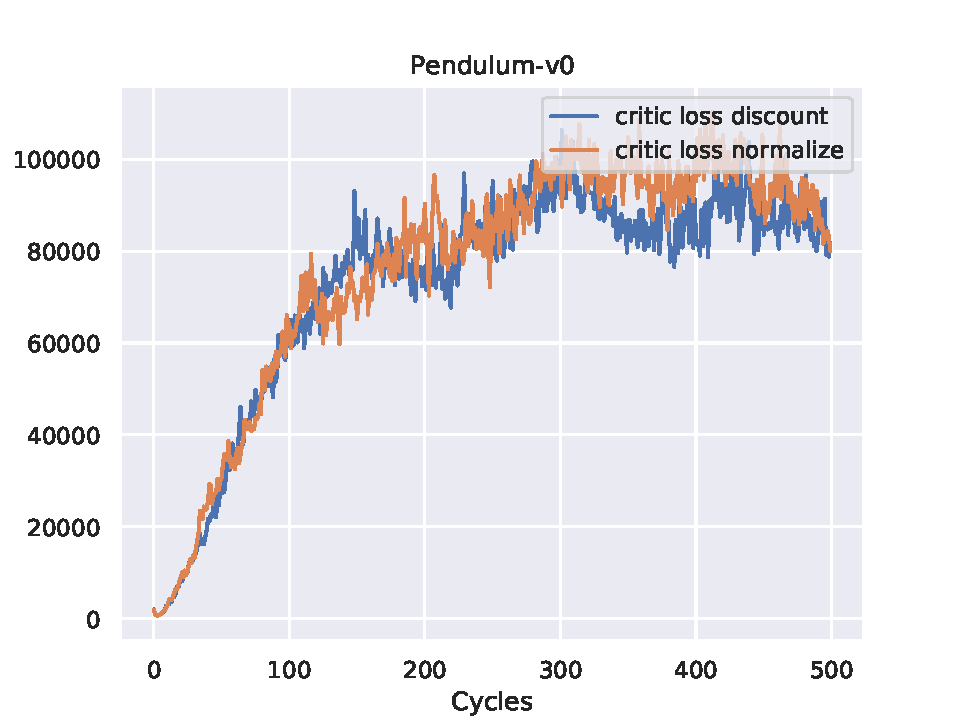
\includegraphics[width=\textwidth]{figures/iteration2/critic_loss_Pendulum-v0_pg_dataset_td_eval_True_cycles_500_trajs_20_batches_20_gamma_0.99_nstep_5_lr_act_0.01_lr_critic_0.01pg.pdf}
        \caption{Fonction de perte de la critique}
    \end{subfigure}
    \begin{subfigure}{0.3\textwidth}
        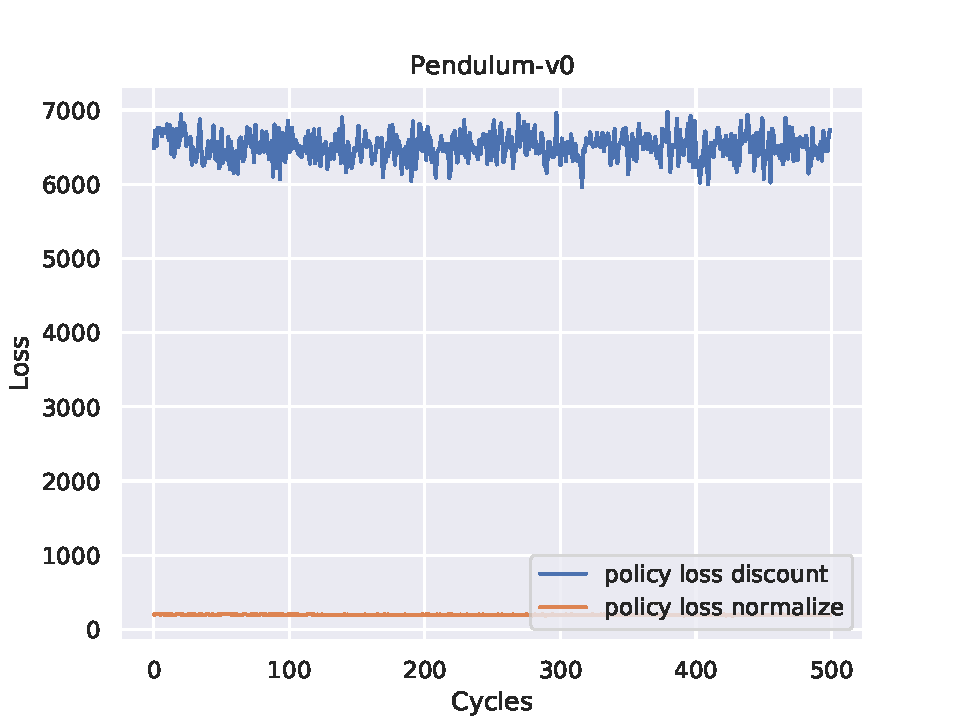
\includegraphics[width=\textwidth]{figures/iteration2/policy_loss_Pendulum-v0_pg_dataset_td_eval_True_cycles_500_trajs_20_batches_20_gamma_0.99_nstep_5_lr_act_0.01_lr_critic_0.01pg.pdf}
        \caption{Fonction de perte de la politique}
    \end{subfigure}
    \begin{subfigure}{0.3\textwidth}
        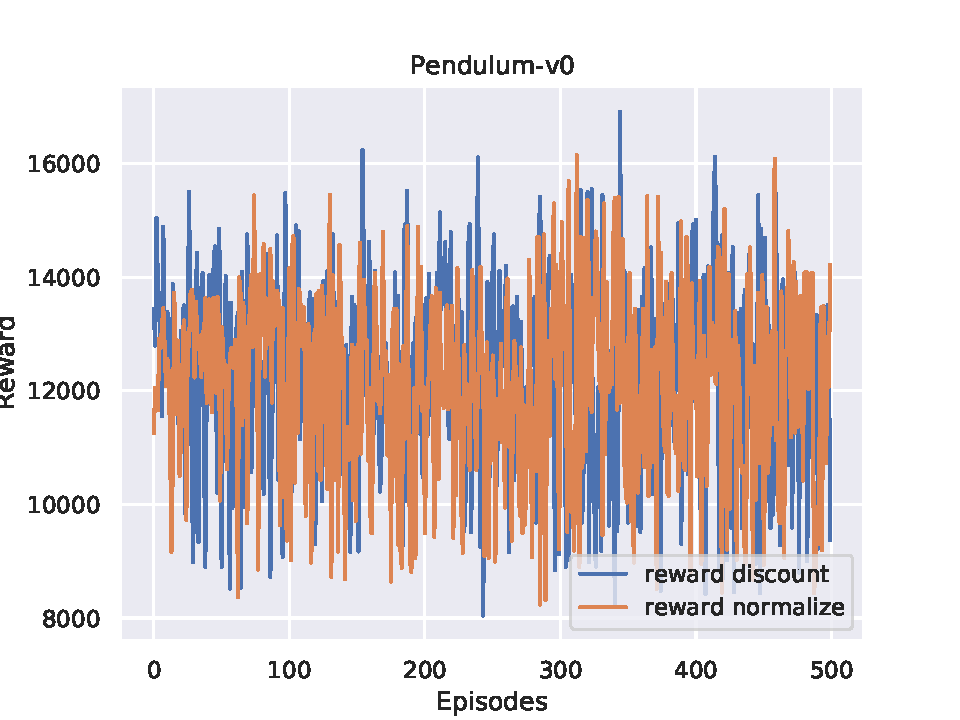
\includegraphics[width=\textwidth]{figures/iteration2/rewards_Pendulum-v0_pg_dataset_td_eval_True_cycles_500_trajs_20_batches_20_gamma_0.99_nstep_5_lr_act_0.01_lr_critic_0.01.pdf}
        \caption{Récompenses des épisodes}
    \end{subfigure}
    \caption{Résultats obtenus pour la critique, la politique et la récompense}
    \label{fig:itr2_results}
\end{figure}

Grâce au redimensionnement de la récompense, les résultats de la figure~\ref{fig:itr2_results} nous montre une convergence de la fonction de perte de la critique bien que très élevé (un peu en dessous des 100 000). On observe également que la fonction de perte est constante pour la méthode \emph{discount} et \emph{normalize}. Mais la perte de la politique obtenue par \emph{normalize} est autour de $100$ et de presque sans bruit. Tandis que celle obtenue par \emph{discount} est très bruitée et se situe autour des $6500$. On aurait donc tendance à croire que la méthode \emph{normalize} doit être favorisée dans le futur. Dans la courbe des récompenses, on n'observe plus de saturation en bas de la courbe comme dans l'itération précédente (voir fig~\ref{fig:attempt1_results}). On peut en déduire qu'il y a plus d'exploration et que le pendule reste moins souvent en bas au cours de tout un épisode.

\begin{figure}[H]
    \centering
    \begin{subfigure}{0.3\textwidth}
        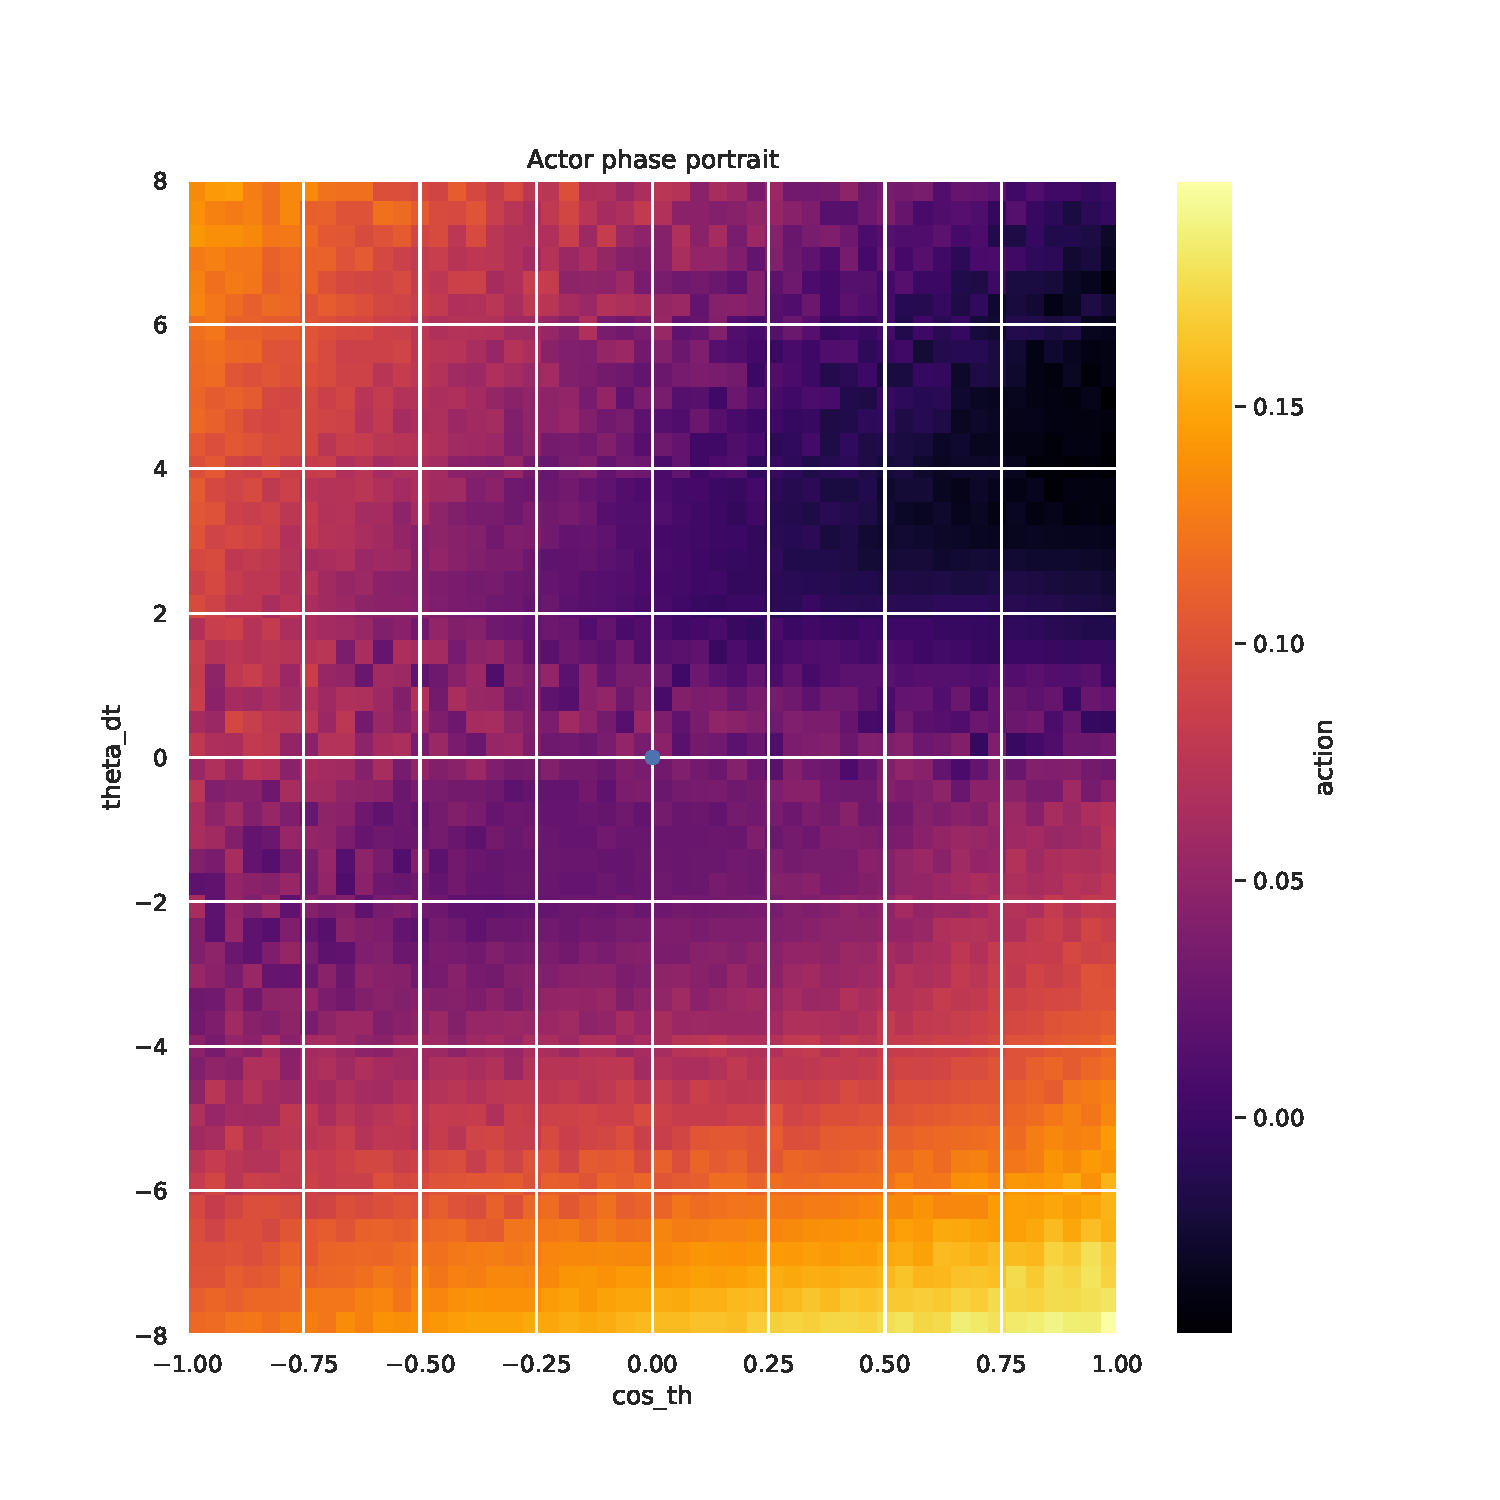
\includegraphics[width=\textwidth]{figures/iteration2/0_actor_discount__ante_Pendulum-v0.pdf}
        \caption{Acteur naïf}
    \end{subfigure}
    \begin{subfigure}{0.3\textwidth}
        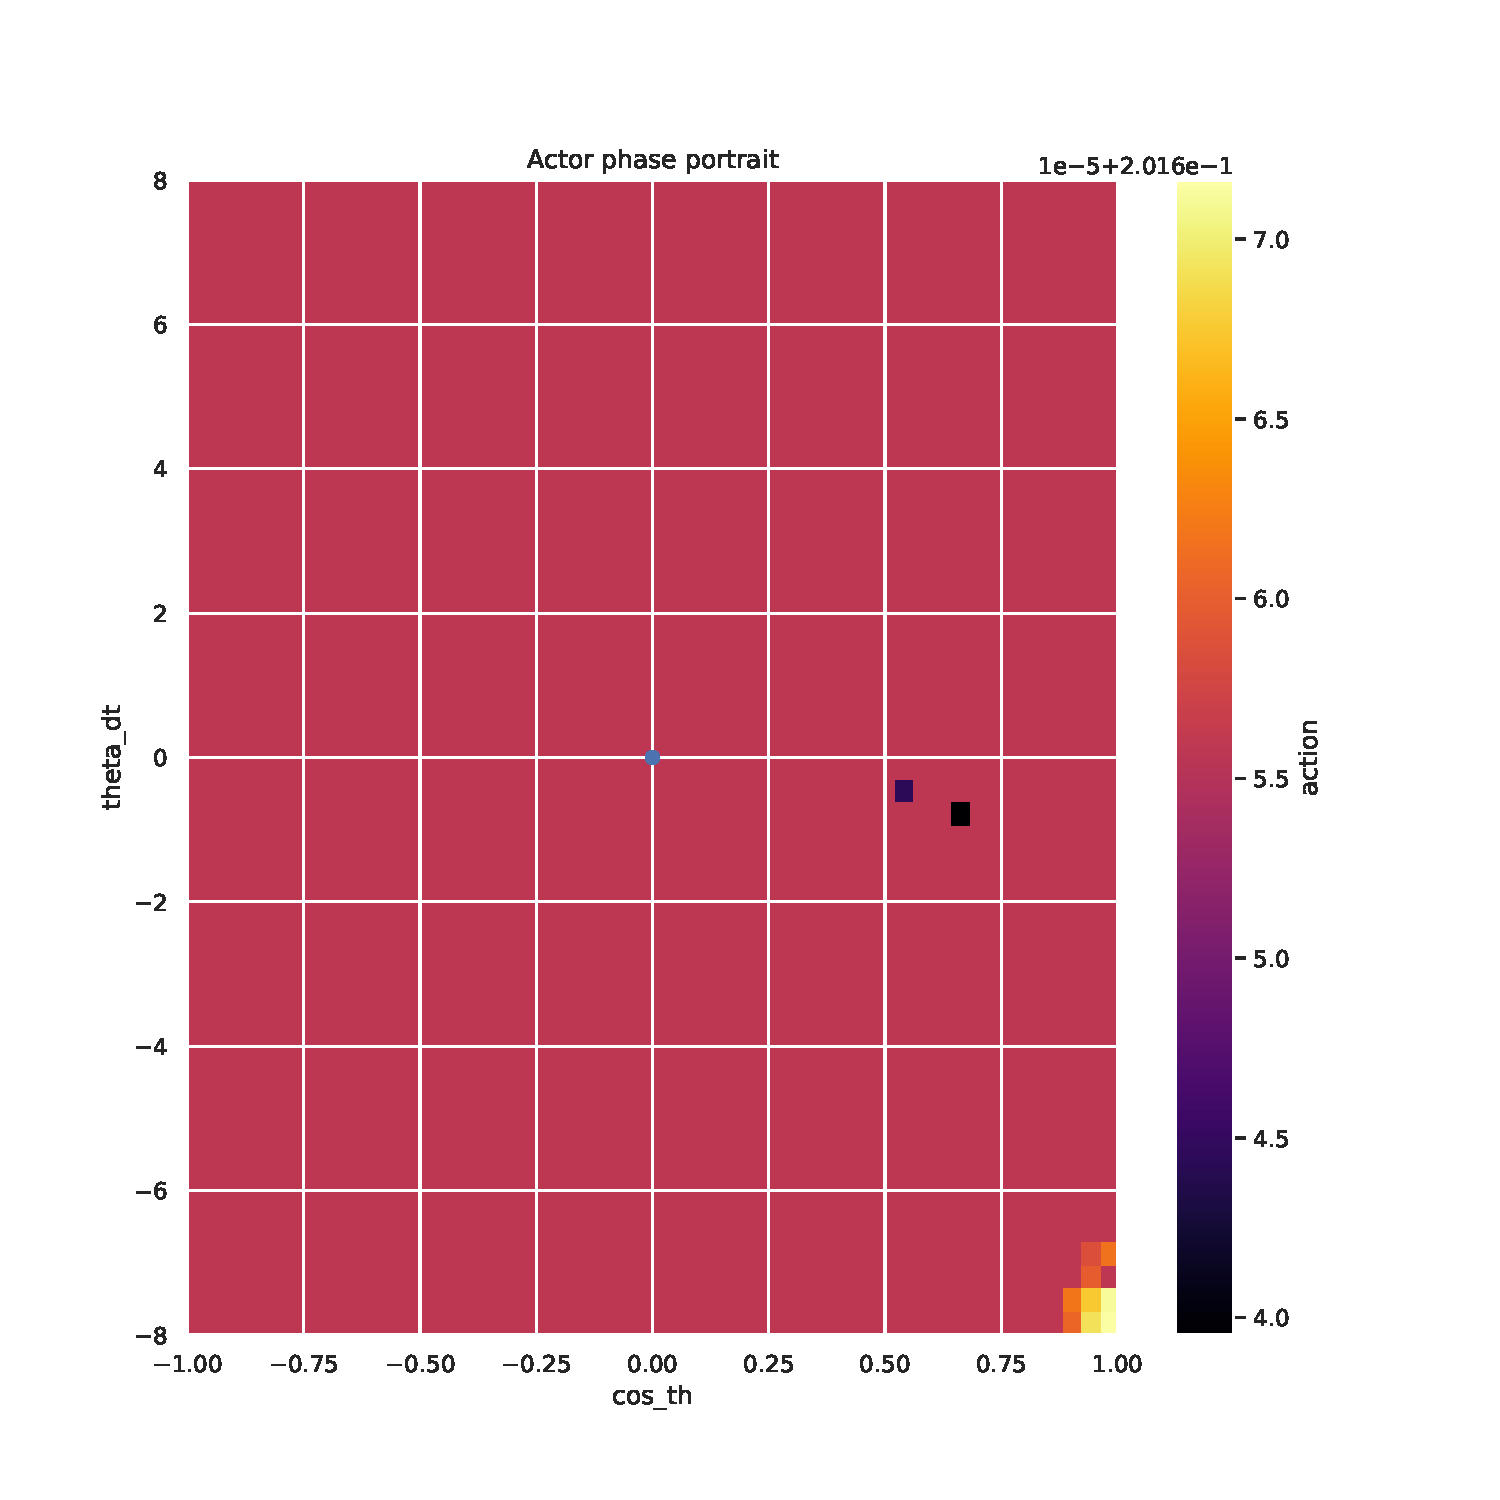
\includegraphics[width=\textwidth]{figures/iteration2/0_actor_discount__post_Pendulum-v0.pdf}
        \caption{Acteur entraîné}
    \end{subfigure}
    \begin{subfigure}{0.3\textwidth}
        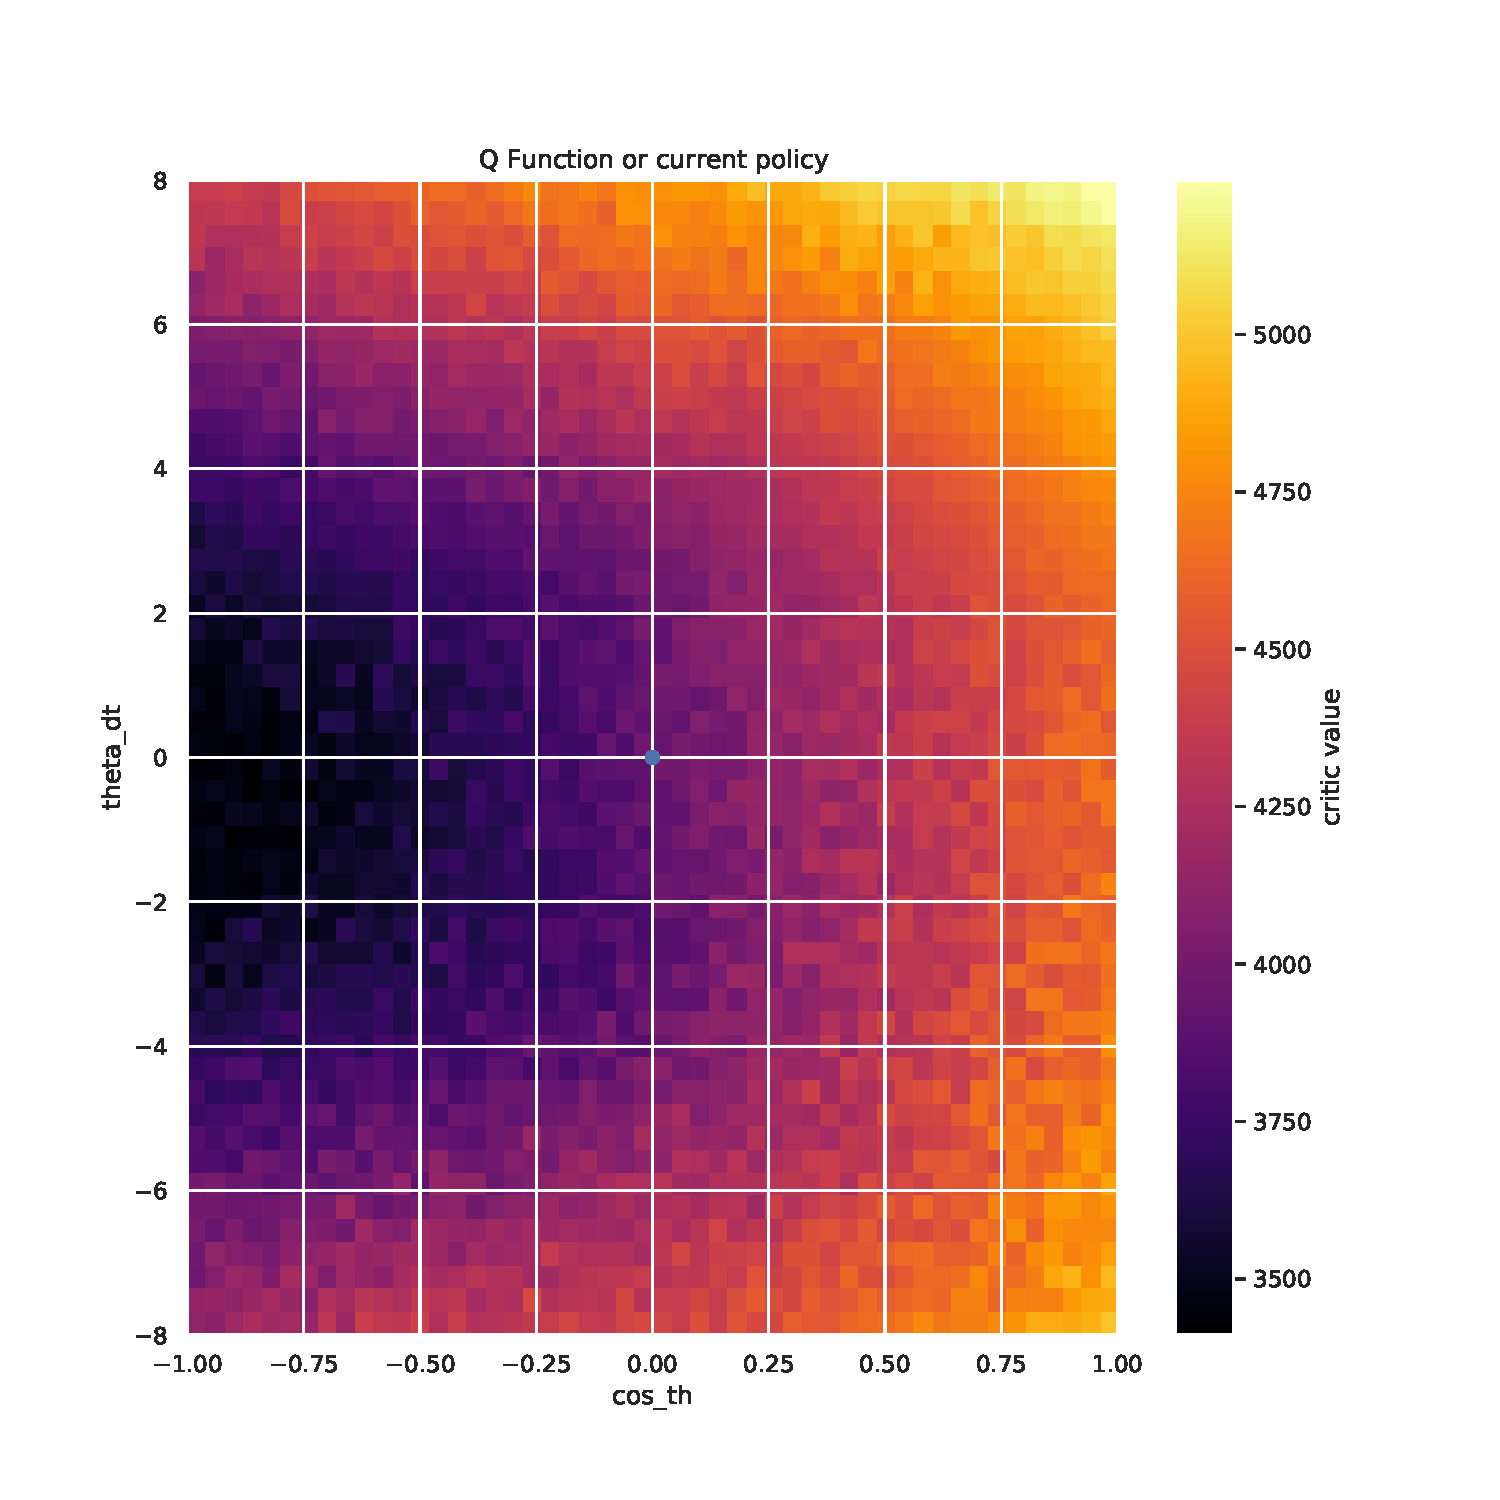
\includegraphics[width=\textwidth]{figures/iteration2/0_critic_discount_post_Pendulum-v0.pdf}
        \caption{Critique entraînée}
    \end{subfigure}
    \caption{Valeurs de l'acteur et de la critique avec la méthode discount pour le calcul de la récompense}
    \label{fig:itr2_discount}
\end{figure}

Dans la figure~\ref{fig:itr2_discount} on retrouve l'acteur uniforme sur l'ensemble des états. De plus, nous ne comprenons pas l'ordre de grandeur de l'échelle des actions. Concernant la critique, elle ne correspond pas à ce qu'on attend car les points clairs sont pour des vitesses angulaires élevées (positive et négative) pour $\cos(\theta) = 1$ alors qu'on voudrait à cette position une vitesse nulle. 

\begin{figure}[H]
    \centering
    \begin{subfigure}{0.3\textwidth}
        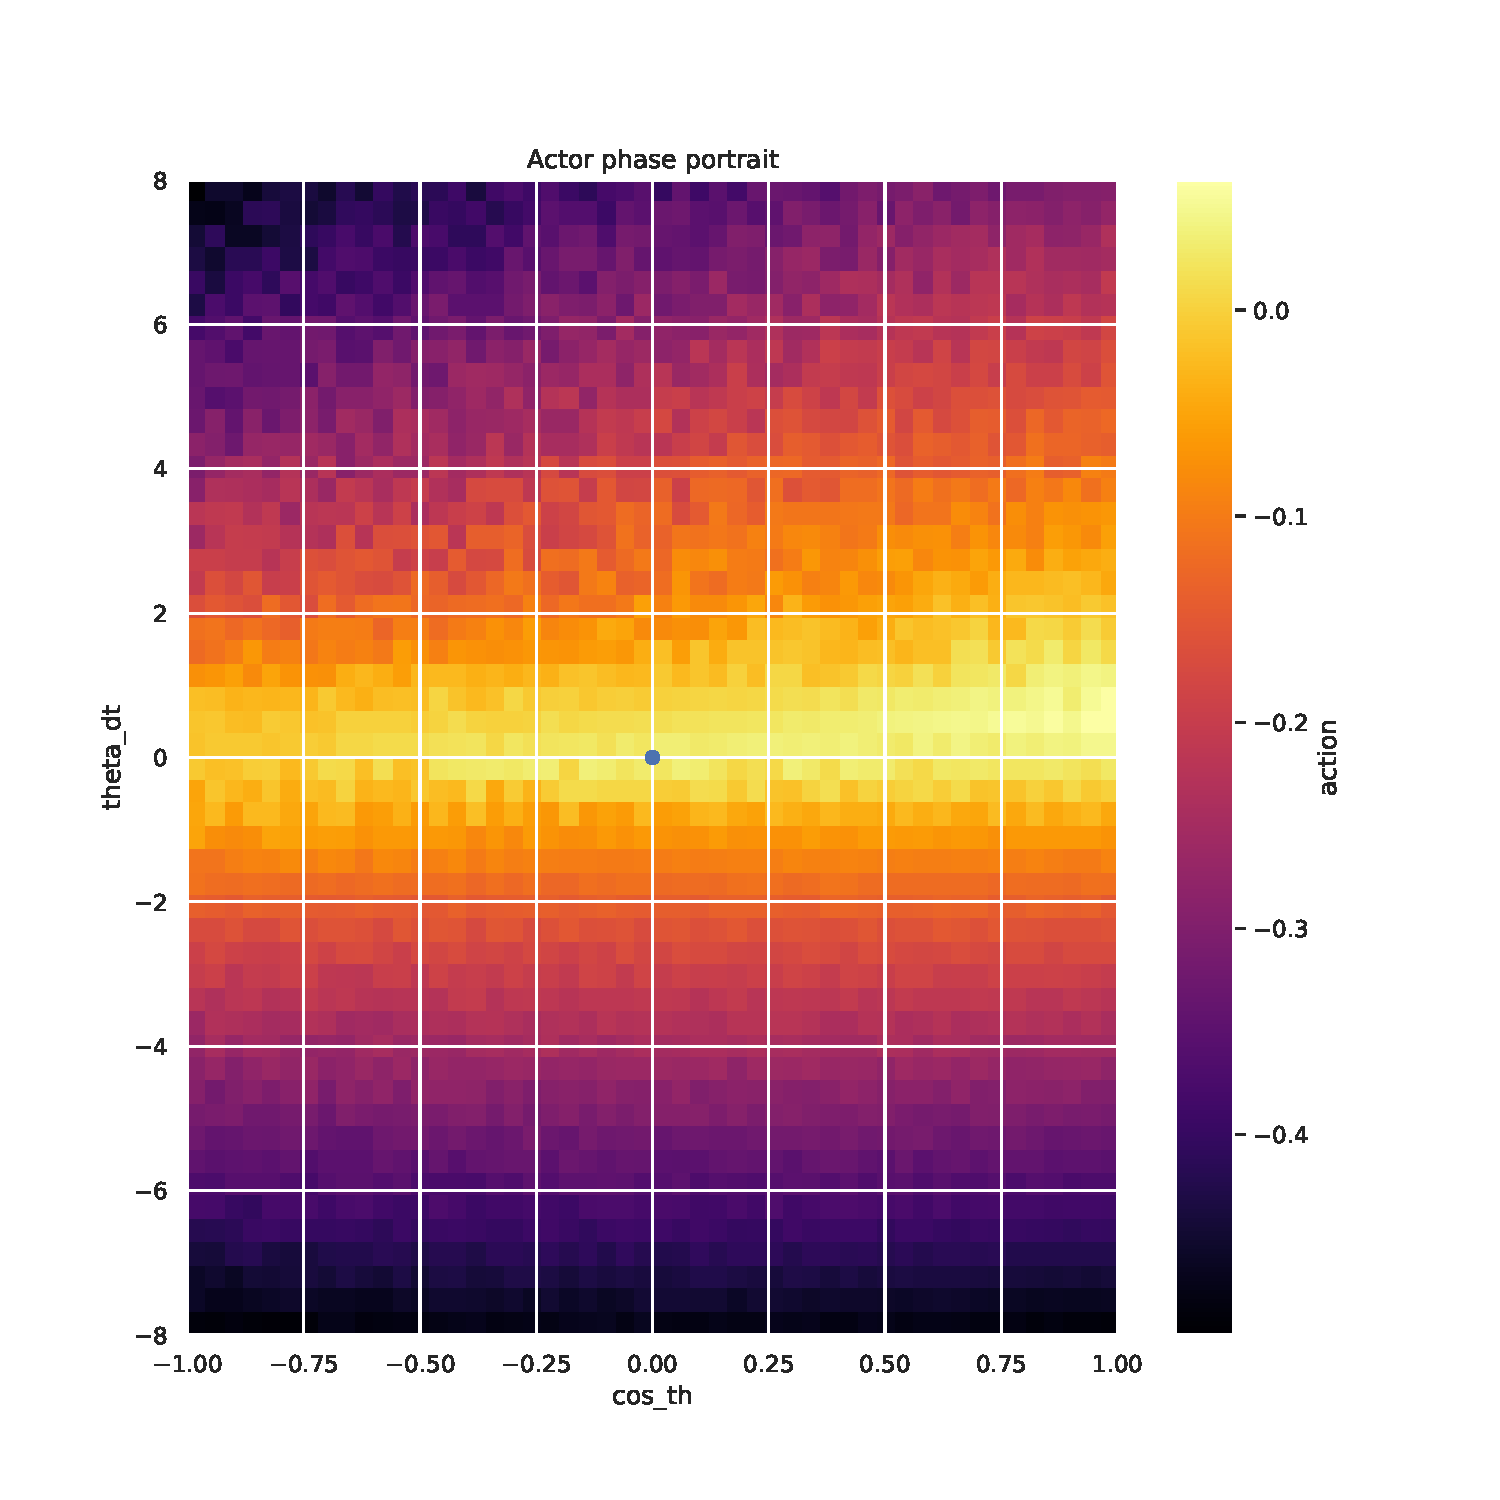
\includegraphics[width=\textwidth]{figures/iteration2/0_actor_normalize__ante_Pendulum-v0.pdf}
        \caption{Acteur naïf}
    \end{subfigure}
    \begin{subfigure}{0.3\textwidth}
        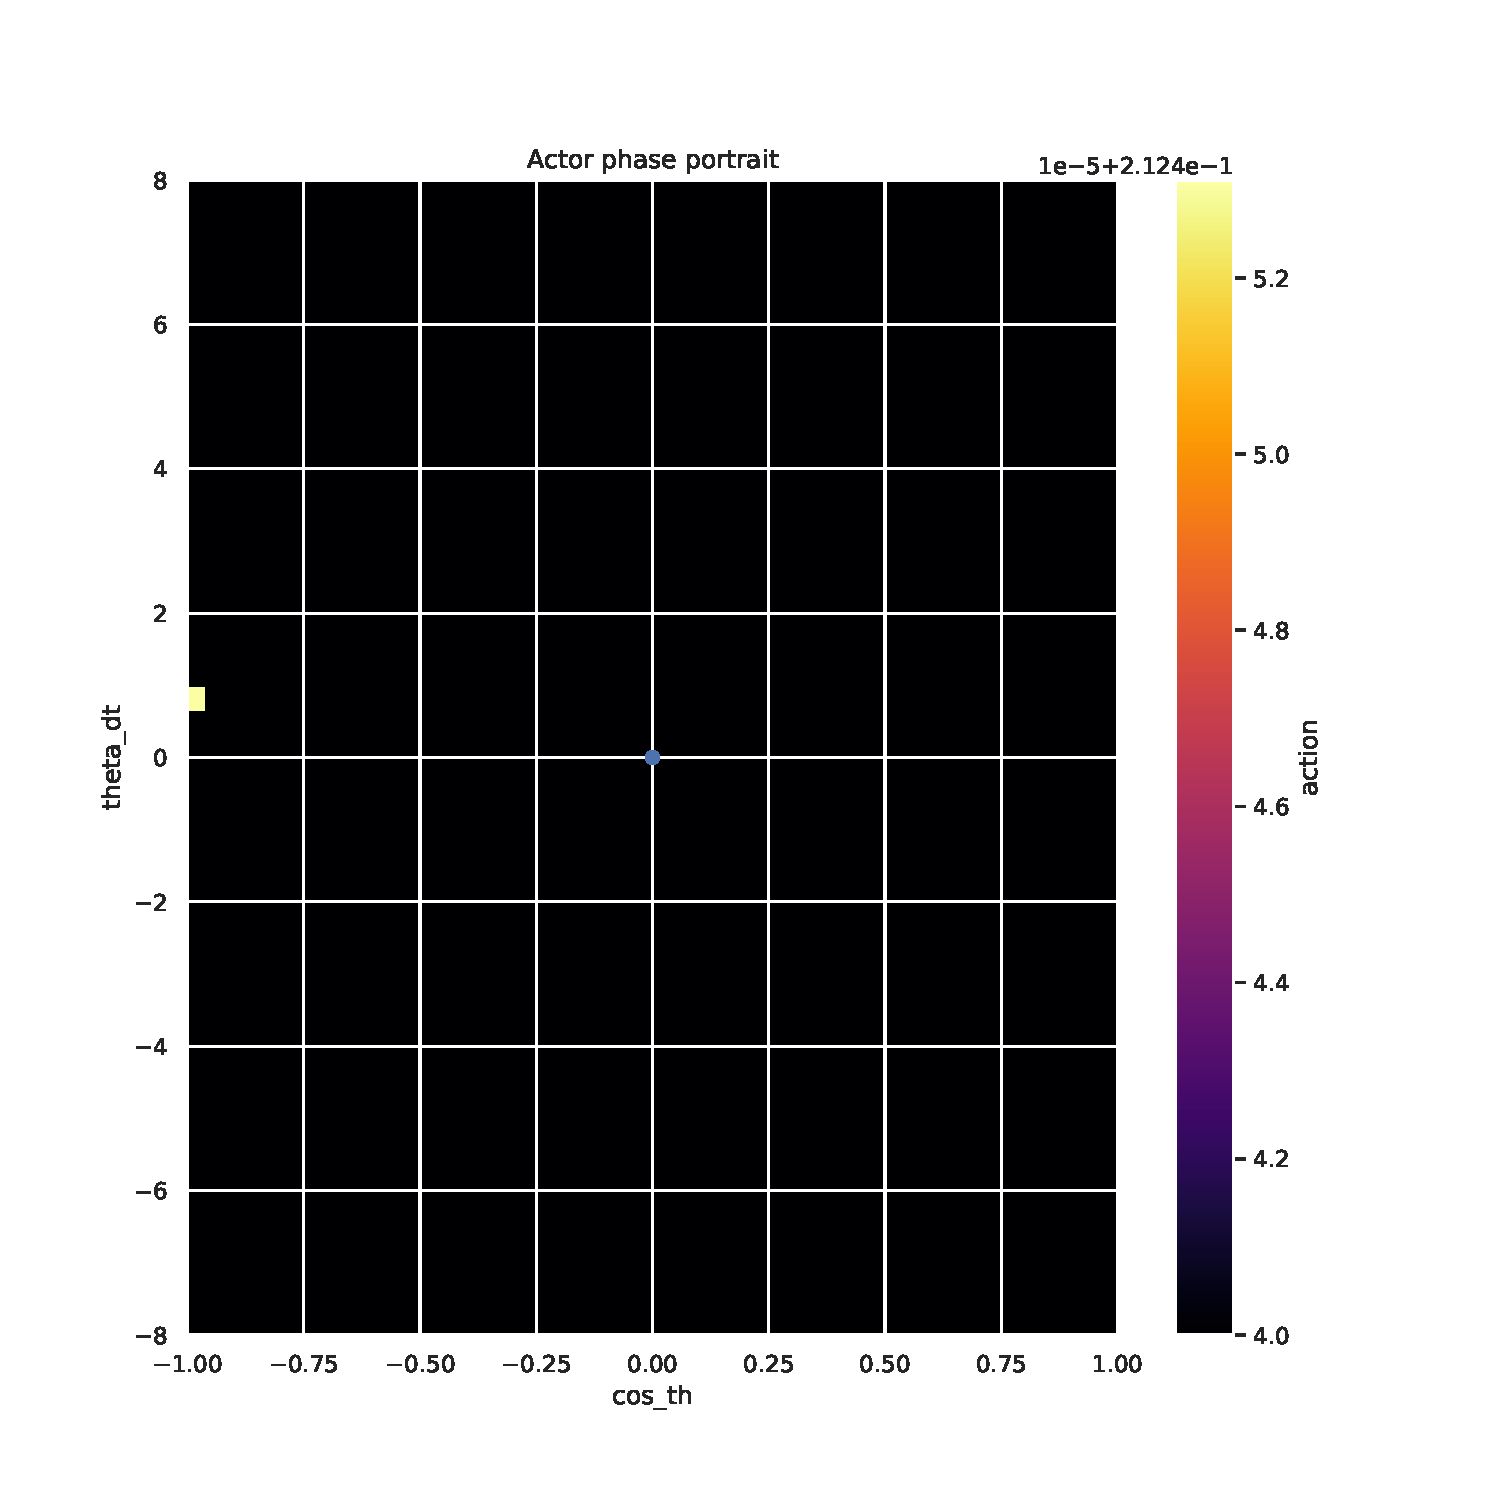
\includegraphics[width=\textwidth]{figures/iteration2/0_actor_normalize__post_Pendulum-v0.pdf}
        \caption{Acteur entraîné}
    \end{subfigure}
    \begin{subfigure}{0.3\textwidth}
        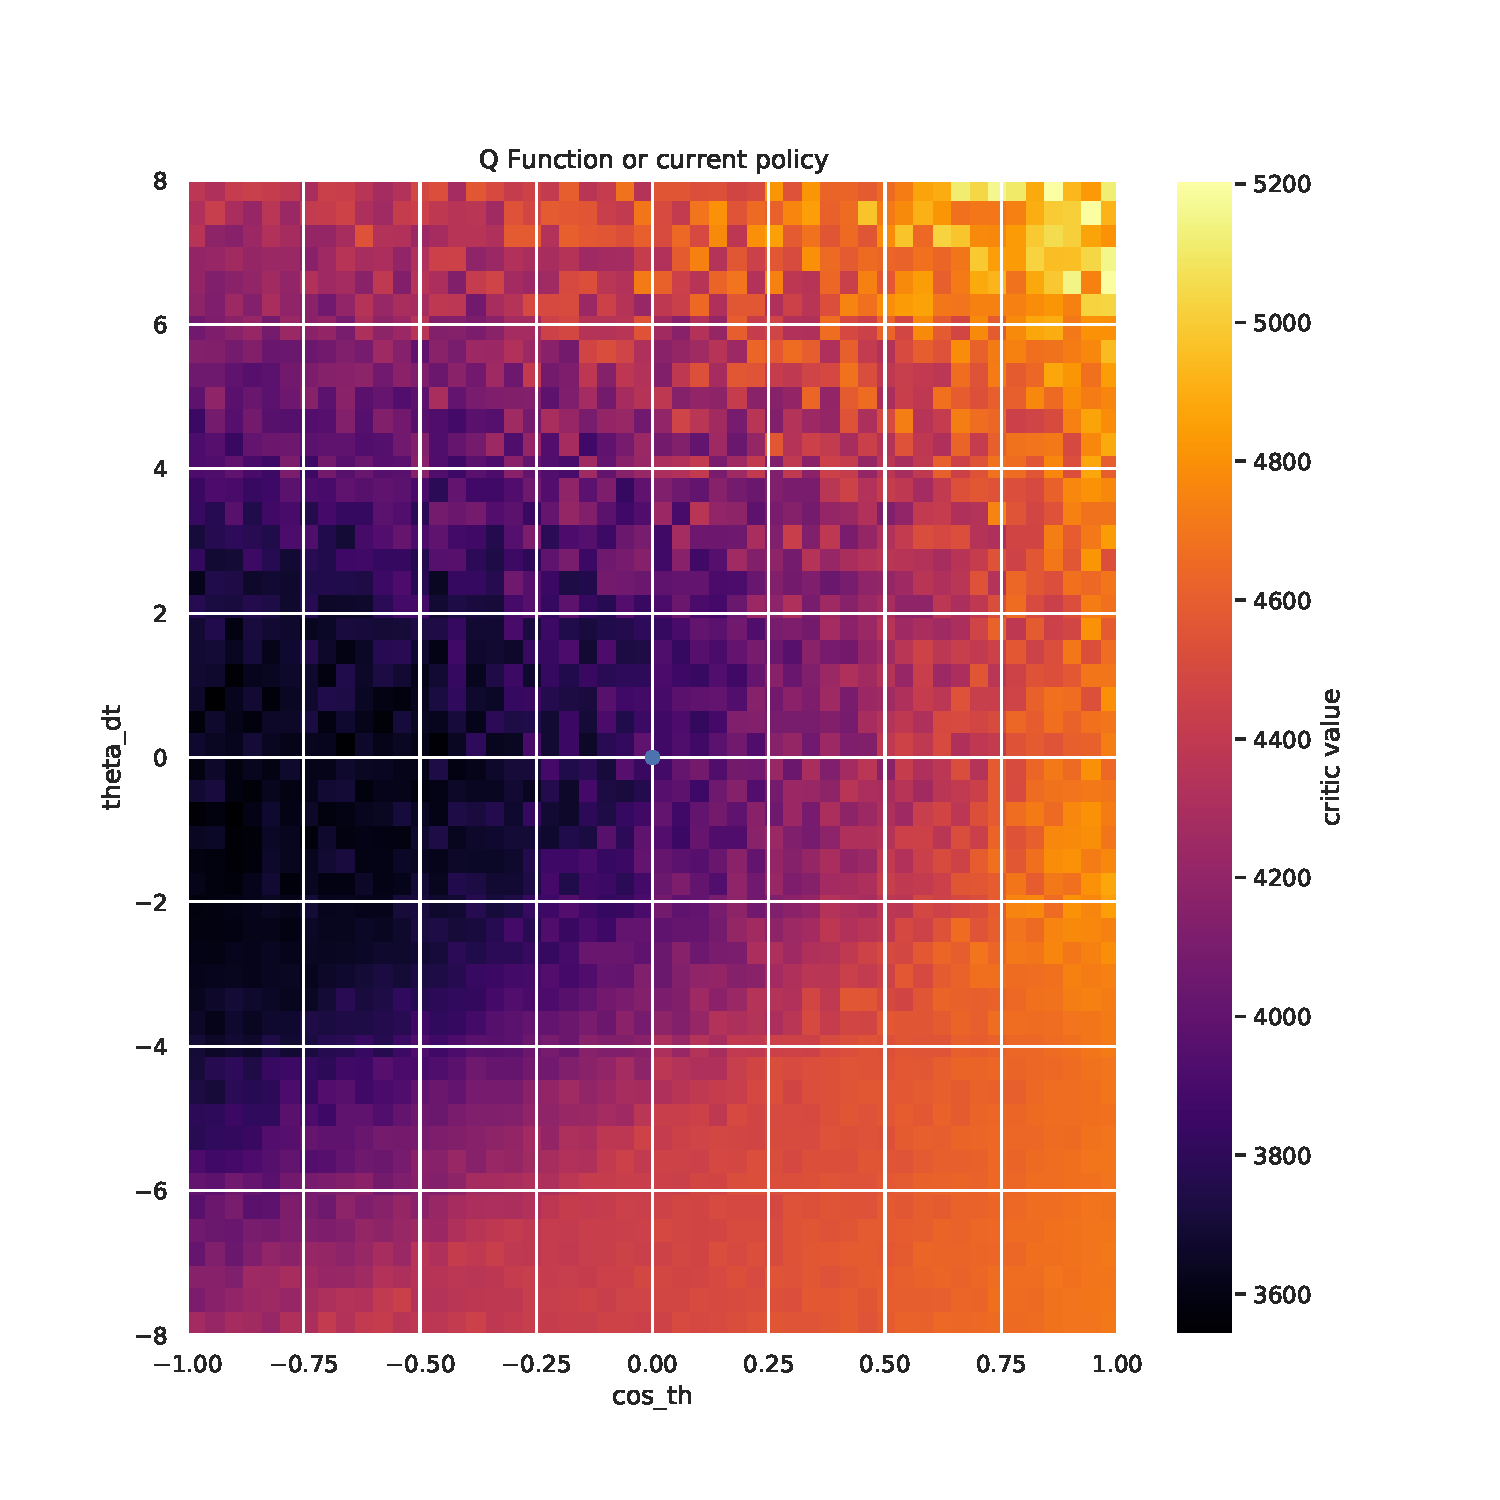
\includegraphics[width=\textwidth]{figures/iteration2/0_critic_normalize_post_Pendulum-v0.pdf}
        \caption{Critique entraînée}
    \end{subfigure}
    \caption{Valeurs de l'acteur et de la critique avec la méthode normalize pour le calcul de la récompense}
    \label{fig:itr2_normalize}
\end{figure}

Ici encore avec la figure~\ref{fig:itr2_normalize} l'acteur entraîné est encore uniforme mais aussi avec un ordre de grandeur incompréhensible sur l'échelle des actions. Comme avec la méthode \emph{discount}, la critique obtenue après apprentissage n'est pas ce que l'on souhaite. Mais pour $\cos(\theta) = -1$ et $\dot{\theta} = 0$ on a bien une zone défavorisée. On peut ainsi comprendre que le pendule évite d'être immobile en bas. Mais pour $\cos(\theta) = 1$ la vitesse à laquelle il se trouve lui importe peu bien qu'il est une préférence pour la vitesse maximale.